\documentclass[12pt,a4paper]{report}
\usepackage[utf8]{inputenc}
\usepackage[francais]{babel}
\usepackage[T1]{fontenc}
\usepackage{amsmath}
\usepackage{amsfonts}
\usepackage{amssymb}
\usepackage{graphicx}
\usepackage{url}
\usepackage{hyperref}
\usepackage[left=2cm,right=2cm,top=2cm,bottom=2cm]{geometry}
\usepackage{listings}
\usepackage{color}

\hypersetup{
backref=true, %permet d'ajouter des liens dans...
pagebackref=true, %...les bibliographies
hyperindex=true, %ajoute des liens dans les index.
colorlinks=true, %colorise les liens
breaklinks=true, %permet le retour à la ligne dans les liens trop longs
urlcolor=red, %couleur des hyperliens
linkcolor=blue, %couleur des liens internes
bookmarks=true, %créé des signets pour Acrobat
bookmarksopen=true, %si les signets Acrobat sont créés,
					%les afficher complètement.
pdftitle={Laboratoire de transmission de signal}, %informations apparaissant dans
pdfauthor={DESSANDE Alexandre, DETOURNAY Jérôme,PECRIAUX Thomas, WERY Michael}, %dans les informations du document
pdfsubject={Fonctionnement du projet} %sous Acrobat.
}

\author{\href{mailto:alex.4492@gmail.com}{Dessandé Alexandre},\href{mailto:jeje.det@gmail.com}{Detournay Jérôme}, \href{mailto:pecriaux.thomas.01@henallux.be}{Pecriaux Thomas}, \href{mailto:wery.michael@gmail.com}{Wery Michael}}
\title{\texttt{\textbf{Laboratoire de transmission de signal}}}

\begin{document}

\definecolor{mygray}{rgb}{0.5,0.5,0.5}

\lstset{
	backgroundcolor=\color{white},   % choose the background color; you must add \usepackage{color} or \usepackage{xcolor}
	basicstyle=\ttfamily,        % the size of the fonts that are used for the code
	breakatwhitespace=false,         % sets if automatic breaks should only happen at whitespace
	breaklines=true,                 % sets automatic line breaking
%	captionpos=b,                    % sets the caption-position to bottom
	commentstyle=\color{green},      % comment style
	deletekeywords={...},            % if you want to delete keywords from the given language
	escapeinside={\%*}{*)},          % if you want to add LaTeX within your code
%	extendedchars=true,              % lets you use non-ASCII characters; for 8-bits encodings only, does not work with UTF-8
	frame=single,                     % adds a frame around the code : single, lines
	keepspaces=true,                 % keeps spaces in text, useful for keeping indentation of code (possibly needs columns=flexible)
	keywordstyle=\color{blue},       % keyword style
	language=C,		                 % the language of the code
	morekeywords={*,...},            % if you want to add more keywords to the set
	numbers=left,                    % where to put the line-numbers; possible values are (none, left, right)
	numbersep=10pt,                  % how far the line-numbers are from the code
	numberstyle=\tiny\color{mygray}, % the style that is used for the line-numbers
	rulecolor=\color{black},         % if not set, the frame-color may be changed on line-breaks within not-black text (e.g. comments (green here))
	showspaces=false,                % show spaces everywhere adding particular underscores; it overrides 'showstringspaces'
	showstringspaces=true,           % underline spaces within strings only
	showtabs=false,                  % show tabs within strings adding particular underscores
	stepnumber=2,                    % the step between two line-numbers. If it's 1, each line will be numbered
	stringstyle=\color{red},         % string literal style
	morecomment=[l][\color{magenta}]{\#},
	tabsize=2,                       % sets default tabsize to 2 spaces
%	title=\lstname                   % show the filename of files included with \lstinputlisting; also try caption instead of title
literate=
  {á}{{\'a}}1 {é}{{\'e}}1 {í}{{\'i}}1 {ó}{{\'o}}1 {ú}{{\'u}}1
  {Á}{{\'A}}1 {É}{{\'E}}1 {Í}{{\'I}}1 {Ó}{{\'O}}1 {Ú}{{\'U}}1
  {à}{{\`a}}1 {è}{{\'e}}1 {ì}{{\`i}}1 {ò}{{\`o}}1 {ò}{{\`u}}1
  {À}{{\`A}}1 {È}{{\'E}}1 {Ì}{{\`I}}1 {Ò}{{\`O}}1 {Ò}{{\`U}}1
  {ä}{{\"a}}1 {ë}{{\"e}}1 {ï}{{\"i}}1 {ö}{{\"o}}1 {ü}{{\"u}}1
  {Ä}{{\"A}}1 {Ë}{{\"E}}1 {Ï}{{\"I}}1 {Ö}{{\"O}}1 {Ü}{{\"U}}1
  {â}{{\^a}}1 {ê}{{\^e}}1 {î}{{\^i}}1 {ô}{{\^o}}1 {û}{{\^u}}1
  {Â}{{\^A}}1 {Ê}{{\^E}}1 {Î}{{\^I}}1 {Ô}{{\^O}}1 {Û}{{\^U}}1
  {œ}{{\oe}}1 {Œ}{{\OE}}1 {æ}{{\ae}}1 {Æ}{{\AE}}1 {ß}{{\ss}}1
  {ç}{{\c c}}1 {Ç}{{\c C}}1 {ø}{{\o}}1 {å}{{\r a}}1 {Å}{{\r A}}1
  {€}{{\EUR}}1 {£}{{\pounds}}1
}
\maketitle
\setcounter{tocdepth}{4}
\tableofcontents

\chapter{Introduction}
	\section{Participants}
		\begin{itemize}
		\item Alexandre Dessandé
		\item Jérôme Detournay
		\item Thomas Pecriaux
		\item Michael Wery
		\end{itemize}
	
	\section{Description du projet}
			Pour notre projet nous avons décidé de faire une application de monitoring pour 
		une salle. Le projet se décompose en deux grandes parties:
		\renewcommand {\labelitemii }{$\diamond $}		
		\begin{itemize}
		\item Une application en \verb+C#+ : 
		Le logiciel reçoit des données du système embarqué et les affiches en temps réel. Nous pourrons
		trouver :
			\begin{itemize}
			\item L'ip de la carte
			\item La température courante, maximum, moyenne.
			\item La luminosité courante, maximum.
			\item La personne connecté.
			\end{itemize}
		Le logiciel pourra aussi faire des actions sur la carte :
			\begin{itemize}
			\item Ajouter des données sur une carte RFID
			\item Allumer ou éteindre une led
			\end{itemize}
		\item Une application en \verb+C+ pour système embarqué :
		Le carte communique avec l'ordinateur via deux méthodes :
			\begin{itemize}
			\item Ethernet
			\item Usart
			\end{itemize}
		Elle possède aussi une communication avec un RFID pour l'authentification sur le logiciel en \verb+C#+.
		\end{itemize}

			
\chapter{Explication des logiciel}
	\section{Description du logiciel C\#}
		\subsection{Introduction}
		Nous allons ici détailler notre application \verb+C#+ pour y parvenir nous décriront en différents points notre logiciel : 
			\begin{itemize}
			\item Connexion: Nous détailleront la connexion au logiciel
			\item Structure du logiciel: Nous parleront de l'agencement graphique
			\item Différentes fonctionnalités: Nous expliqueront les différentes parties du logiciel
			\end{itemize}
		\subsection{Connexion}
		Lors de l'ouverture du logiciel une fenêtre d'authentification s'ouvre, celle-ci  vous demande de passer votre carte RFID pour vous logguer au programme. Ceci fait vous arrivez sur la page principale du logiciel.
		\subsection{Structure du logiciel}
		\begin{center}
		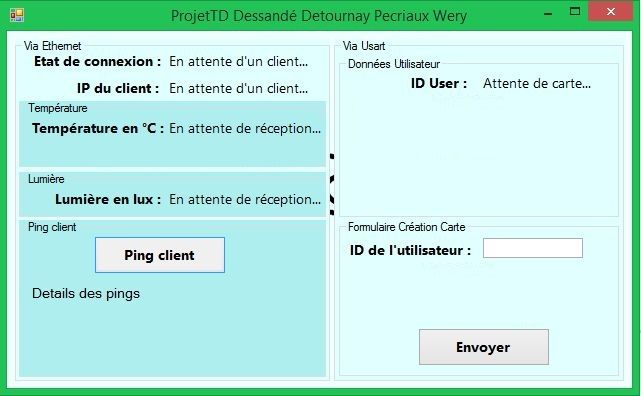
\includegraphics[scale=0.6]{ImageElec.jpg}
		\end{center}
		
		
		\subsection{Différentes fonctionnalités}
			\paragraph{Données Ethernet:}S'il n'y a pas de client connecté il nous affiche "En attente d'un client" dans les deux partie sinon :
			\begin{itemize}
			\item pour l'état de connexion il affiche "Client connecté" 
			\item pour l'IP il affichera l'IP du système embarqué			
			\end{itemize}
			\paragraph{Température:}Nous pouvons trouver dans cette partie la température actuelle si aucune donnée n'a encore été récupérée il affiche : "En attende de données".
			\paragraph{Luminosité:}Nous pouvons trouver dans cette partie la luminosité dans la pièce si aucune donnée n'a encore été récupérée il affiche : "En attende de données".
			\paragraph{Client:}Cette partie nous donne les informations concernant la personne qui c'est connecté au logiciel via une carte RFID.
			\paragraph{Création de carte:}A partir d'ici nous pouvons remplir un petit formulaire pour écrire sur une carte RFID.
			\paragraph{Ping:}La section ping dispose d'un bouton où lorsque l'on clique dessus nous pourront voir s'afficher les différentes données du ping : 
			\begin{itemize}
			\item Si réussit ou non
			\item L'ip du client
			\item le TTL
			\item La fragmentation des données sur plusieurs
			\item La taille du buffer
			\end{itemize}
			Si la carte est éteint le bouton renverrai un "Time Out"
			\paragraph{Erreur socket:} Lorsque l'on le câble Ethernet est retiré le programme nous sort une erreur.
	
	\section{Description du logiciel C}
	Nous parlons ici notre application \verb+C+ mis en place sur notre système embarqué.  
		\subsection{Introduction}
		\subsection{Ethernet}
		\subsection{Usart}
		\subsection{RFID}
	
			\begin{lstlisting}

			\end{lstlisting}

\end{document}